\subsection{Photon-Gluon Fusion}

Given the relatively small lever arm in $Q^2$ currently available to constrain
$\Delta G$ via evolution of $g_1$, it is natural to pursue an alternative
approach involving observables that are directly linked to the gluon
polarization. In photon-gluon fusion (PGF), the lepton emits a real or virtual
photon that interacts with a gluon radiated from the nucleon to produce a
$q\bar{q}$ pair (see Figure \ref{fig:pgf}). PGF is a rare process compared to
scattering off of quarks in the nucleon, and as such analyses need a way to
enhance the signal to background ratio. The golden signature for PGF is charm
in the final state, since the nucleon itself has a negligible charm content.
Charm production has a small cross section, so analyses that look for
high-$p_T$ final states are also common.

Figure \ref{fig:pgf-deltag} summarizes results for the gluon polarization
extracted at leading order from analyses of photon-gluon fusion processes.
SMC, HERMES, and COMPASS have all released results based on the detection of
high-$p_T$ hadrons or jets, and COMPASS has released a single data point from
an analysis of charmed ($D^0$ and $D^*$) mesons. The data cover an $x$ range
of approximately $0.07 < \langle x \rangle < 0.2$ and restrict the magnitude
of the gluon polarization within that region. No NLO analysis of PGF data on
$\Delta G$ is currently available.

\begin{figure}
  \centering
  \begin{fmfgraph*}(200,150)
    \fmfleft{proton,gamma}
    \fmfright{proton',quark1,quark2}
    \fmf{fermion,width=2.5}{proton,v1}
    \fmf{fermion}{v1,proton'}
    \fmf{gluon}{v1,v2}
    \fmfblob{.15w}{v1}
    \fmf{fermion}{v2,quark1}
    \fmf{fermion}{v2,v3,quark2}
    \fmf{photon}{gamma,v3}

    % wow, it really feels like I should not have to do all of this
    \fmffixedx{0.}{v2,v3}
    \fmffixedy{0.}{v2,quark1}
    \fmffixedy{0.}{v3,quark2}
    \fmffixedy{0.}{v1,proton'}
    \fmffreeze
    \fmfshift{(0,-0.2h)}{v3}
    \fmfshift{(0.09w,-0.2h)}{quark2}
    \fmfshift{0,0.15h}{v1,proton'}
    
    % finally, add lines for outgoing quarks in struck proton
    \fmfi{plain}{vpath (__v1, __proton') shifted (thick*(-0.5,3.5))}
    \fmfi{plain}{vpath (__v1, __proton') shifted (thick*(-0.5,-3.5))}
  \end{fmfgraph*}
  \caption{Feynman diagram of photon-gluon fusion process}
  \label{fig:pgf}
\end{figure}


\begin{figure}
  \centering
  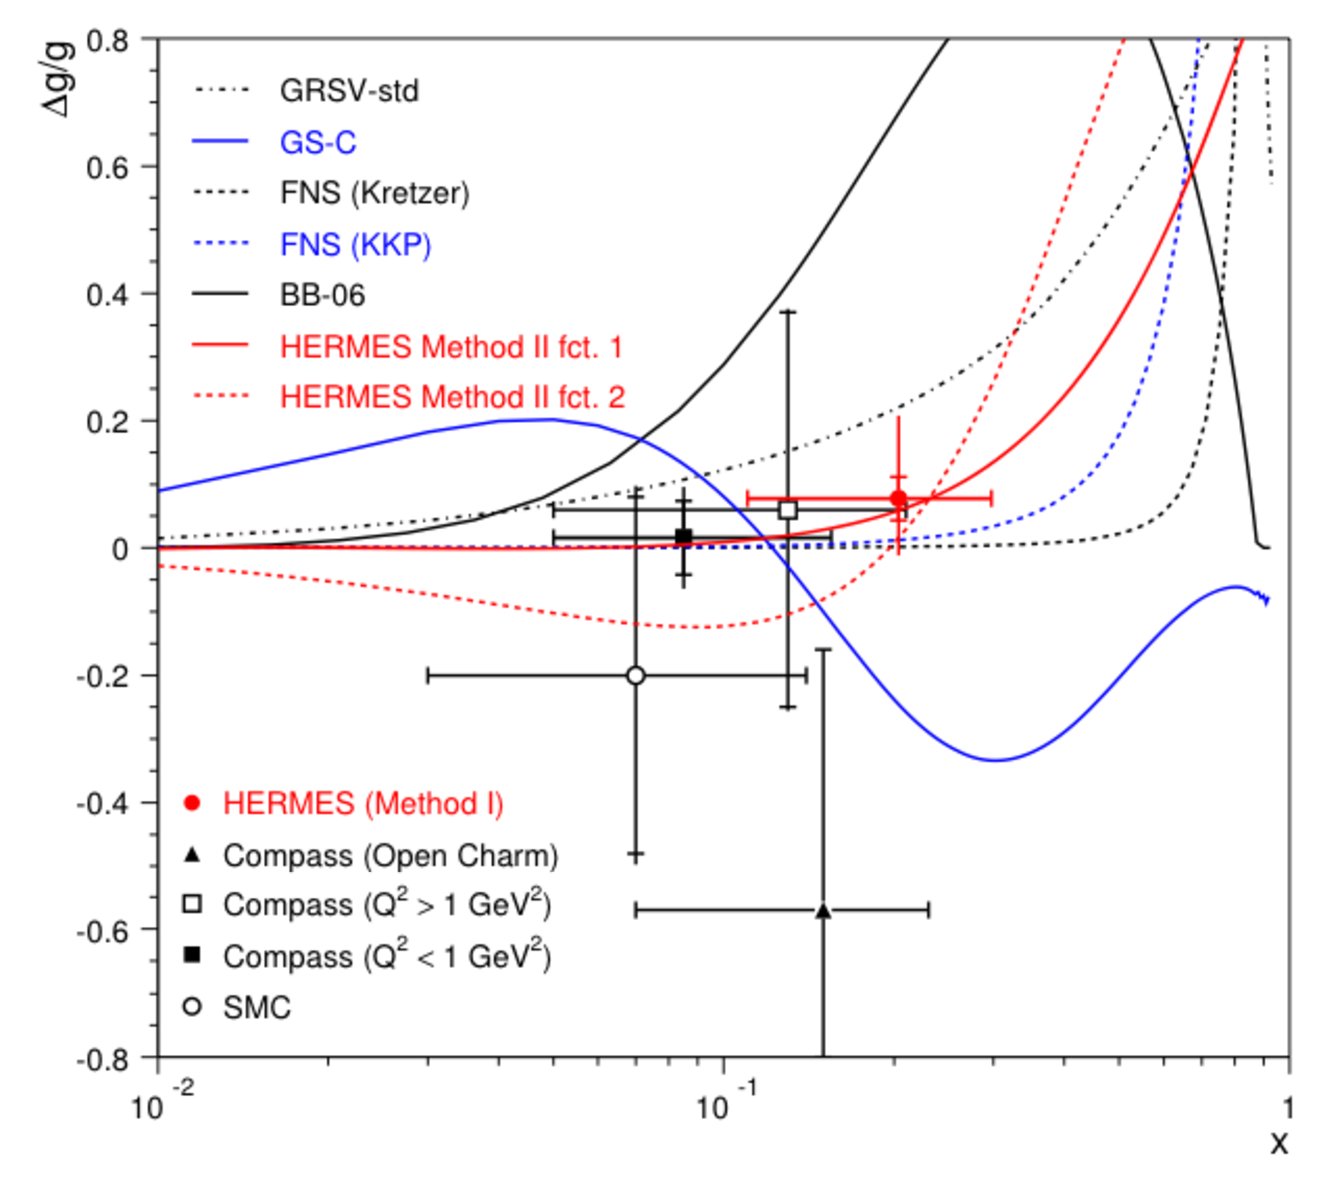
\includegraphics[width=0.7\textwidth]{figures/dgg-hermes-final}
  \caption{Compilation of $\Delta g(x)/g(x)$ measurements from SMC, HERMES,
  and COMPASS plotted versus momentum fraction \cite{Hasch:2009zza}.}
  \label{fig:pgf-deltag}
\end{figure}

% ... this is wrong, the number is just for the COMPASS open charm measurement, the most recent LO global analysis from COMPASS yields $\Delta g(x)/g(x) = -0.49~\pm~0.27~(stat)~\pm~0.11~(syst)$ at a scale $\mu^2 \sim 13~(GeV/c)^2$ and at an average gluon momentum fraction $\langle x \rangle ~\sim 0.11$ \cite{Alekseev:2009ey}.

%% Direct \Delta G figure without preliminary results
% \begin{figure}
%   \includegraphics[width=1.0\textwidth]{figures/compass_deltag}
%   \caption{\cite{Alekseev:2009ey}}
% \end{figure}
